\bta{探究加速度与物体质量、物体受力的关系}
\begin{enumerate}
\renewcommand{\labelenumi}{\arabic{enumi}.}
% A(\Alph) a(\alph) I(\Roman) i(\roman) 1(\arabic)
%设定全局标号series=example	%引用全局变量resume=example
%[topsep=-0.3em,parsep=-0.3em,itemsep=-0.3em,partopsep=-0.3em]
%可使用leftmargin调整列表环境左边的空白长度 [leftmargin=0em]
\item
\exwhere{$ 2013 $ 年天津卷}
某实验小组利用图示的装置探究加速度
打点计时器
与力、质量的关系。
\begin{figure}[h!]
\centering
\includesvg[width=0.63\linewidth]{picture/svg/GZ-3-tiyou-0530}
\end{figure}



①下列做法正确的是 \tk{AD} (填字母代号)
\fourchoices
{调节滑轮的高度,使牵引木块的细绳与长木板保持平行}
{在调节木板倾斜度平衡木块受到的滑动摩擦力时,将装有砝码的砝码桶通过定滑轮拴木块上}
{实验时,先放开木块再接通打点计时器的电源}
{通过增减木块上的砝码改变质量时,不需要重新调节木板倾斜度}

②为使砝码桶及桶内砝码的总重力在数值上近似等于木块运动时受到的拉力,应满足的条件是砝码
桶及桶内砝码的总质量
\tk{远小于} 
木块和木块上砝码的总质量(填“远大于”、“远小于”或“近似等于”)


③甲、乙两同学在同一实验室,各取一套图示的装置放在水平桌面上,木块上均不放砝码,在没有
平衡摩擦力的情况下,研究加速度 $ a $ 与拉力 $ F $ 的关系,分别得到图中甲、
乙两条直线。设甲、乙用的木块质量分别为 $ m_{ \text{甲} } $ 、$ m_{ \text{乙} } $ ,甲、乙用的木块
与木板间的动摩擦因数分别为$ \mu_{ \text{甲} } $,$ \mu_{ \text{乙} } $,由图可知,$ m_{ \text{甲} } $ 
\tk{小于} 
$ m $ 乙,
$ \mu_{ \text{甲} } $
\tk{大于} 
$ \mu $乙。(填“大于”、“小于”或“等于”)
\begin{figure}[h!]
\centering
\includesvg[width=0.23\linewidth]{picture/svg/GZ-3-tiyou-0531}
\end{figure}



\newpage
\item 
\exwhere{$ 2013 $ 年四川卷}
如图 $ 1 $ 所示,某组同学借用“探究 $ a $ 与 $ F $、$ m $ 之间的定量关系”的相关实验思想、原理及操作,
进行“研究合外力做功和动能变化的关系”的实验:
\begin{figure}[h!]
\centering
\includesvg[width=0.93\linewidth]{picture/svg/GZ-3-tiyou-0532}
\end{figure}




①为达到平衡阻力的目的,取下细绳及托盘,通过调整垫片的位置,改变长木板倾斜程度,根据打
出的纸带判断小车是否做 \tk{匀速} 运动。


②连接细绳及托盘,放入砝码,通过实验得到图 $ 2 $ 所示的纸带。纸带上 $ O $ 为小车运动起始时刻所打
的点,选取时间间隔为 $ 0.1 \ s $ 的相邻计数点 $ A $、$ B $、$ C $、$ D $、$ E $、$ F $、$ G $。实验时小车所受拉力为 $ 0.2 \ N $,
小车的质量为 $ 0.2 \ kg $。


请计算小车所受合外力做的功 $ W $ 和小车动能的变化$ \Delta E_{k} $,补填表中空格(结果保留至小数点后第四
位)
。


\begin{table}[h!]
\centering 
\begin{tabular}{|c|c|c|c|c|c|}
\hline 
& $ O-B $
& $ O-C $ & $ O-D $ & $ O-E $

& $ O-F $
\\
\hline
$ W/J $ & $ 0.0432 $ & $ 0.0572 $ & $ 0.0734 $ & $ 0.0915 $ & \tk{$ 0.1115 $} 
\\
\hline
$ \Delta E_{k} /J $ & $ 0.0430 $ & $ 0.0570 $ & $ 0.0734 $ & $ 0.0907 $ & \tk{$ 0.1105 $} \\ 
\hline 
\end{tabular}
\end{table} 


分析上述数据可知:在实验误差允许的范围内 $ W= \Delta E_{k} $,与理论推导结果一致。

③实验前已测得托盘质量为 $ 7.7 \times 10^{-3} \ kg $,实验时该组同学放入托盘中的砝码质量应为 \tk{0.015} $ kg $
($ g $ 取 $ 9.8 \ m/s^{2} $,结果保留至小数点后第三位)。


\newpage
\item
\exwhere{$ 2014 $ 年理综新课标$ \lmd{1} $卷}
某同学利用图$ (a) $所示实验装置及数字化信息系统获得了小车加速度 $ a $ 与钩码的质量 $ m $ 的对应
关系图,如图$ (b) $所示。实验中小车(含发射器)的质量为 $ 200 \ g $,实验时选择了不可伸长的轻质细
绳和轻定滑轮,小车的加速度由位移传感器及与之相连的计算机得到,回答下列问题:
\begin{figure}[h!]
\centering
\includesvg[width=0.83\linewidth]{picture/svg/GZ-3-tiyou-0533}
\end{figure}

\begin{enumerate}
\renewcommand{\labelenumi}{\arabic{enumi}.}
% A(\Alph) a(\alph) I(\Roman) i(\roman) 1(\arabic)
%设定全局标号series=example	%引用全局变量resume=example
%[topsep=-0.3em,parsep=-0.3em,itemsep=-0.3em,partopsep=-0.3em]
%可使用leftmargin调整列表环境左边的空白长度 [leftmargin=0em]
\item
根据该同学的结果,小车的加速度与钩码的质量成\tk{非线性}(选填“线性”或“非线性”)关系.



\item 
由图$ (b) $可知,$ a-m $ 图线不经过原点,可能的原因是 \tk{存在摩擦力} .




\item 
若利用本实验装置来验证“在小车质量不变的情况下,小车的加速度与作用力成正比”的结论,并
直接以钩码所受重力 $ mg $ 作为小车受到的合外力,则实验中应采取的改进措施是 \tk{调整轨道倾斜度以平衡摩擦力} ,钩码的
质量应满足的条件是 \tk{远小于小车质量} .


\end{enumerate}






\item
\exwhere{$ 2011 $ 年理综浙江卷}
在“探究加速度与力、质量的关系”实验时,已提
供了小车,一端附有定滑轮的长木板、纸带、带小盘的细线、
刻度尺、天平、导线。为了完成实验,还须从下图中选取实验
器材,其名称是 \tk{学生电源、电磁打点计时器、钩码、砝码或电火花计时器、钩码、砝码} 
(漏选或全选得
零分);并分别写出所选器材的作用 \tk{学生电源为电磁打点计时器提供交流电源;电磁打点计时器(电火花计时器)记录小车运动的位
置和时间;钩码用以改变小车的质量;砝码用以改变小车受到的拉力的大小,还可以用于测量小车
的质量}。
% TODO: \usepackage{graphicx} required
\begin{figure}[h!]
\centering
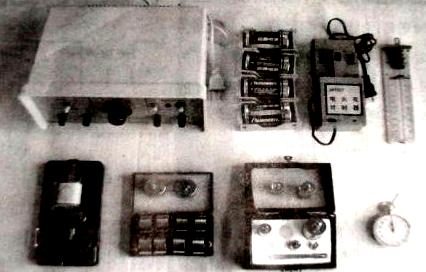
\includegraphics[width=0.4\linewidth]{picture/screenshot033}
\end{figure}




\newpage
\item
\exwhere{$ 2012 $ 年理综全国卷}
图 $ 1 $ 为验证牛顿第二定律的实验装置示意图。图中打点计时器的电源为 $ 50 \ Hz $ 的交流电源,打
点的时间间隔用$ \Delta t $ 表示。在小车质量未知的情况下,某同学设计了一种方法用来研究“在外力一
定的条件下,物体的加速度与其质量间的关系”。
\begin{figure}[h!]
\centering
\includesvg[width=0.63\linewidth]{picture/svg/GZ-3-tiyou-0534}
\end{figure}





\begin{enumerate}
\renewcommand{\labelenumi}{\arabic{enumi}.}
% A(\Alph) a(\alph) I(\Roman) i(\roman) 1(\arabic)
%设定全局标号series=example	%引用全局变量resume=example
%[topsep=-0.3em,parsep=-0.3em,itemsep=-0.3em,partopsep=-0.3em]
%可使用leftmargin调整列表环境左边的空白长度 [leftmargin=0em]
\item
完成下列实验步骤中的填空:



①平衡小车所受的阻力:小吊盘中不放物块,调整木
板右端的高度,用手轻拨小车,直到打点计时器打出
一系列 \tk{间距相等} 的点。

②按住小车,在小吊盘中放入适当质量的物块,在小
车中放入砝码。


③打开打点计时器电源,释放小车,获得带有点列的纸带,在纸带上标出小车中砝码的质量 $ m $。


④按住小车,改变小车中砝码的质量,重复步骤③。


⑤在每条纸带上清晰的部分,每 $ 5 $ 个间隔标注一个计数点。测量相邻计数点的间距 $ s_{1} $,$ s_{2} $,$ \cdots $。求
出与不同 $ m $ 相对应的加速度 $ a $。



⑥以砝码的质量 $ m $ 为横坐标,
$\frac{1}{a}$为纵坐标,在坐标纸上作出 $\frac{1}{a}-m$ 关系图线。若加速度与小车和
砝码的总质量成反比,则
$\frac{1}{a}$
与 $ m $ 应成 \tk{线性} 关系(填“线性”或“非线性”)。


\item 
完成下列填空:
\begin{enumerate}
\renewcommand{\labelenumiii}{\roman{enumiii}.}
% A(\Alph) a(\alph) I(\Roman) i(\roman) 1(\arabic)
%设定全局标号series=example	%引用全局变量resume=example
%[topsep=-0.3em,parsep=-0.3em,itemsep=-0.3em,partopsep=-0.3em]
%可使用leftmargin调整列表环境左边的空白长度 [leftmargin=0em]
\item
本实验中,为了保证在改变小车中砝码的质量时,小车所受的拉力近似不变,小吊盘和盘中
物块的质量之和应满足的条件是 \tk{远小于小车和小车中砝码的质量之和} 。


\item 
设纸带上三个相邻计数点的间距为 $ s_{1} $、$ s_{2} $、$ s_{3} $。$ a $ 可用 $ s_{1} $、$ s_{3} $ 和$ \Delta t $ 表
示为 $ a= $ \tk{$\frac{s_{3}-s_{1}}{2(5 \Delta t)^{2}}=\frac{s_{3}-s_{1}}{50(\Delta t)^{2}}$} 。图 $ 2 $ 为用米尺测量某一纸带上的 $ s_{1} $、$ s_{3} $ 的情况,由图
可 读 出 $ s_{1}= $ \tk{$36.6-12.5=24.1 \mathrm{mm}$} , $ s_{3}= $ \tk{$=120-72.7=47.3 \mathrm{mm}$} 。 由 此 求 得 加 速 度 的 大 小
$ a=$ \tk{$ 1.16 $} $m/s^{2} $。
\begin{figure}[h!]
\centering
\includesvg[width=0.83\linewidth]{picture/svg/GZ-3-tiyou-0535}
\end{figure}

\item 
图 $ 3 $ 为所得实验图线的示意图。设图中直线的斜率为 $ k $,在纵轴上的
截距为 $ b $,若牛顿定律成立,则小车受到的拉力为 \tk{$ \frac{1}{k} $} ,小车的质量为 \tk{$ \frac{b}{k} $} 。
\begin{figure}[h!]
\centering
\includesvg[width=0.2\linewidth]{picture/svg/GZ-3-tiyou-0536}
\end{figure}


\end{enumerate}


\end{enumerate}


\newpage
\item 
\exwhere{$ 2012 $ 年理综安徽卷}
图 $ 1 $ 为“验证牛顿第二定律”的实验装置示意图。砂和砂桶的总质量为 $ m $,小车和砝码的总质量为
$ M $。实验中用砂和砂桶总重力的大小作为细线对小车拉力的大小。
\begin{figure}[h!]
\centering
\includesvg[width=0.43\linewidth]{picture/svg/GZ-3-tiyou-0537}
\end{figure}

\begin{enumerate}
\renewcommand{\labelenumi}{\arabic{enumi}.}
% A(\Alph) a(\alph) I(\Roman) i(\roman) 1(\arabic)
%设定全局标号series=example	%引用全局变量resume=example
%[topsep=-0.3em,parsep=-0.3em,itemsep=-0.3em,partopsep=-0.3em]
%可使用leftmargin调整列表环境左边的空白长度 [leftmargin=0em]
\item
实验中,为了使细线对小车的拉力等于小车所受的合外力,先调节长木板一端滑轮的高度,使细
线与长木板平行。接下来还需要进行的一项操作是 \tk{B} 。 


\threechoices
{将长木板水平放置,让小车连着已经穿过打点计时器的纸带,给打点计时器通电,调节 $ m $ 的大小,使小车在砂和砂桶的牵引下运动,从打出的纸带判断小车是否做匀速运动。}
{将长木板的一端垫起适当的高度,让小车连着已经穿过打点计时器的纸带,撤去砂和砂桶,给打点计时器通电,轻推小车,从打出的纸带判断小车是否做匀速运动。}
{将长木板的一端垫起适当的高度,撤去纸带以及砂和砂桶,轻推小车,观察判断小车是否做匀速运动。}


\item 
实验中要进行质量 $ m $ 和 $ M $ 的选取,以下最合理的一组是 \tk{C}。 
\fourchoices
{$ M=20 \ g ,m=10 \ g $、$ 15 \ g $、$ 20 \ g $、$ 25 \ g $、$ 30 \ g $、$ 40 \ g $}
{$ M=200 \ g ,m=20 \ g $、$ 40 \ g $、$ 60 \ g $、$ 80 \ g $、$ 100 \ g $、$ 120 \ g $}
{$ M=400 \ g ,m=10 \ g $、$ 15 \ g $、$ 20 \ g $、$ 25 \ g $、$ 30 \ g $、$ 40 \ g $}
{$ M=400 \ g ,m=20 \ g 40 \ g $、$ 60 \ g $、$ 80 \ g $、$ 100 \ g $、$ 120 \ g $}

\item 
图 $ 2 $ 是实验中得到的一条纸带,
$ A $、 $ B $、$ C $、 $ D $、 $ E $、 $ F $、$ G $ 为 $ 7 $ 个
相邻的计数点,相邻的两个计数点之间
还有四个点未画出。量出相邻的计数点
之间的距离分别为 $ s_{AB}=4.22 \ cm $、 $ s_{BC}=4.65 \ cm $、 $ s_{CD}=5.08 \ cm $、 $ s_{DE}=5.49 \ cm $、 $ s_{EF}=5.91 \ cm $、
$ s_{FG}=6.34 \ cm $。已知打点计时器的工作频率为 $ 50 \ Hz $,则小车的加速度 $ a= $
\tk{$ 0.42 $} 
$ m/s^{2} $ (结果
保留 $ 2 $ 位有效数字)。
\begin{figure}[h!]
\centering
\includesvg[width=0.63\linewidth]{picture/svg/GZ-3-tiyou-0538}
\end{figure}


\end{enumerate}



\newpage
\item 
\exwhere{$ 2016 $ 年新课标$ \lmd{3} $卷}
某物理课外小组利用图($ a $)中的装置探究物体加速度与其所受
合外力之间的关系。图中,置于实验台上的长木板水平放置,其右端固定一轻滑轮:轻绳跨过滑轮,
一端与放在木板上的小滑车相连,另一端可悬挂钩码。本实
验中可用的钩码共有 $ N=5 $ 个,每个质量均为 $ 0.010 \ kg $。实验步
骤如下:
\begin{figure}[h!]
\centering
\includesvg[width=0.33\linewidth]{picture/svg/GZ-3-tiyou-0539}
\end{figure}

\begin{enumerate}
\renewcommand{\labelenumi}{\arabic{enumi}.}
% A(\Alph) a(\alph) I(\Roman) i(\roman) 1(\arabic)
%设定全局标号series=example	%引用全局变量resume=example
%[topsep=-0.3em,parsep=-0.3em,itemsep=-0.3em,partopsep=-0.3em]
%可使用leftmargin调整列表环境左边的空白长度 [leftmargin=0em]
\item
将 $ 5 $ 个钩码全部放入小车中,在长木板左下方垫上适当
厚度的小物快,使小车(和钩码)可以在木板上匀速下滑。


\item 
将 $ n $(依次取 $ n=1,2,3,4,5 $)个钩码挂在轻绳右端,其余 $ N-n $ 各钩码仍留在小车内;用手按住小
车并使轻绳与木板平行。释放小车,同时用传感器记录小车在时刻 $ t $ 相对于其起始位置的位移 $ s $,
绘制 $ s-t $ 图像,经数据处理后可得到相应的加速度 $ a $。
\begin{figure}[h!]
\centering
\includesvg[width=0.83\linewidth]{picture/svg/GZ-3-tiyou-0540}
\end{figure}



\item 
对应于不同的 $ n $ 的 $ a $ 值见下表。$ n=2 $ 时的 $ s-t $ 图像如图($ b $)所示:由图($ b $)求出此时小车的
加速度(保留 $ 2 $ 位有效数字),将结果填入下表。
\begin{table}[h!]
\centering 
\begin{tabular}{|c|c|c|c|c|c|}
\hline 
$ n $ & $ 1 $ & $ 2 $ & $ 3 $ & $ 4 $ & $ 5 $
 \\
\hline
$ a/m \cdot s^{-2} $ & $ 0.20 $ & \tk{$ 0.39 $} & $ 0.58 $ & $ 0.78 $ & $ 1.00 $\\ 
\hline 
\end{tabular}
\end{table} 





\item 
利用表中的数据在图($ c $)中补齐数据点,并作出 $ a-n $ 图像。从图像可以看出:当物体质量一
定时,物体的加速度与其所受的合外力成正比。
\banswer{
 \includesvg[width=0.23\linewidth]{picture/svg/GZ-3-tiyou-0541} 
}

\item 
利用 $ a $–$ n $ 图像求得小车(空载)的质量为 \tk{$ 0.45 $} $ kg $(保留 $ 2 $ 位有效数字,重力加速度取 $ g=9.8 \ m \cdot s ^{-2}$)。

\item 
若以“保持木板水平”来代替步骤($ 1 $),下列说法正确的是 \tk{BC} (填入正确选项钱的标号)
\threechoices
{$ a - n $ 图线不再是直线}
{$ a - n $ 图线仍是直线,但该直线不过原点}
{$ a - n $ 图线仍是直线,但该直线的斜率变大}

\end{enumerate}



\banswer{

}




\end{enumerate}

